\documentclass[conference]{IEEEtran}
\IEEEoverridecommandlockouts
\usepackage{cite}
\usepackage{amsmath,amssymb,amsfonts}
\usepackage{algorithmic}
\usepackage{graphicx}
\usepackage{textcomp}
\usepackage{xcolor}
\usepackage{booktabs}
\usepackage{multirow}
\usepackage{array}
\usepackage{comment}
\usepackage{url}
\usepackage{hyperref}
\def\BibTeX{{\rm B\kern-.05em{\sc i\kern-.025em b}\kern-.08em
    T\kern-.1667em\lower.7ex\hbox{E}\kern-.125emX}}

\begin{document}

\title{When Does Test-Time Adaptation Fail for Multi-Instance Learning? A Diagnostic Study on Breast Cancer Histopathology}

\makeatletter
\newcommand{\linebreakand}{%
  \end{@IEEEauthorhalign}
  \hfill\mbox{}\par
  \mbox{}\hfill\begin{@IEEEauthorhalign}
}
\makeatother


\author{
\IEEEauthorblockN{Akib Hasan Pyil}
\IEEEauthorblockA{
\textit{Department of Computer Science} \\
\textit{American International University-Bangladesh} \\
Dhaka, Bangladesh \\
23-50531-1@student.aiub.edu
}
\and
\IEEEauthorblockN{Mohammad Rabib Uddin}
\IEEEauthorblockA{
\textit{Department of Electrical and Electronic Engineering} \\
\textit{American International University-Bangladesh} \\
Dhaka, Bangladesh \\
rabib@aiub.edu
}
}
 
\maketitle

\begin{abstract}
Test-time adaptation (TTA) has reduced distribution-shift errors by up to 40\% on natural image benchmarks, motivating its application to computational pathology, where cross-site generalization remains a persistent deployment problem. We apply four TTA strategies --- TENT (entropy minimization), TTT (self-supervised auxiliary task), CORAL (covariance alignment), and a phased Hybrid --- to Multi-Instance Learning (MIL) aggregators trained on the BACH breast histopathology dataset and evaluated on BreakHis without target labels. On BACH, UNI-based AB-MIL reaches 0.9700 accuracy and 0.9973 AUROC across five folds. Despite this strong source performance, none of the TTA methods improve cross-domain accuracy on BreakHis beyond the no-adaptation baseline. A supervised fine-tuning upper bound reaches 0.9250 accuracy with the same features, confirming that the features are suitable and the failure belongs to the adaptation mechanism itself. We trace this failure to a fundamental precondition violation: BACH trains a 4-class classifier while BreakHis requires a 2-class one, so the classification head is randomly re-initialized at transfer time. TTA updates only LayerNorm affine parameters and cannot recover a randomly initialized head. This result identifies a critical precondition --- label-space compatibility between source and target --- that must hold for TTA to function in MIL settings, and provides concrete guidance for practitioners deploying MIL models across institutions.
\end{abstract}

\begin{IEEEkeywords}
test-time adaptation, multi-instance learning, breast cancer histopathology, domain generalization, pathology foundation models, negative result, weakly supervised learning
\end{IEEEkeywords}

\section{Introduction}

Computational pathology models do not travel well. A MIL classifier trained on slides from one institution commonly loses five to twenty percentage points when evaluated on slides from another, due to scanner differences, staining variation, and demographic shifts \cite{chen2022scaling, lu2021data}. This is not a theoretical concern --- it is a routine obstacle to clinical deployment, and it happens even when the underlying task is identical at both sites.

Test-time adaptation (TTA) is a compelling response to this problem. TTA updates a small subset of model parameters at inference time using only the unlabeled test sample. It requires no target-domain labels, no retraining, and no access to source data beyond what was already baked into the trained model. On natural image corruption benchmarks, TENT \cite{wang2021tent} reduces classification error by up to 40\%, and more recent methods push further \cite{niu2023towards, liu2021ttt}. The promise is real: label-free adaptation at test time, with no retraining cost.

Applying TTA to MIL introduces complications that the TTA literature has not addressed. In standard image classification, TTA processes one image per call. In MIL, the inference unit is a bag of patches --- typically 32 to thousands per slide. Bag-level entropy is noisier than single-image entropy. The attention aggregator introduces a pooling step that TTA was not designed around. The feature dimensionality is high. None of these properties is obviously favorable for entropy minimization or covariance alignment.

Despite all this, the pathology community has not yet asked systematically whether TTA works for MIL, under what conditions, and why it might fail. This paper provides that study. We implement TENT, TTT, CORAL, and a phased Hybrid TTA strategy for three MIL aggregators (AB-MIL \cite{ilse2018attention}, TransMIL \cite{shao2021transmil}, CLAM \cite{lu2021data}) trained on BACH \cite{aresta2019bach} with ResNet-50 and UNI \cite{chen2024uni} features, and evaluate cross-domain transfer to BreakHis \cite{spanhol2016dataset}. The result is a null: TTA produces no meaningful improvement in this setting.

The more important contribution is the diagnosis. We trace the failure to a precondition that TTA literature takes for granted --- label-space compatibility between source and target. BACH is 4-class; BreakHis is binary. The classification head is replaced and randomly re-initialized at transfer time, and TTA, updating only LayerNorm affine parameters, has no path to recover a random output layer. A supervised fine-tuning upper bound with 30\% labeled target samples reaches 0.9250 accuracy, confirming the features are rich enough and the failure is structural.

This result matters because the same setup --- a source model with a different label space from the target, a replaced head, and a hope that unsupervised adaptation will bridge the gap --- is common in practice. Clarifying why this fails, and what preconditions TTA requires to work, is useful to anyone deploying MIL models across sites.

The contributions of this paper are:

\begin{enumerate}
    \item \textbf{First systematic TTA study for MIL:} Four TTA strategies are adapted and implemented for MIL aggregators operating on pre-extracted patch features, across two feature backbones and three aggregator architectures.

    \item \textbf{Rigorous null result with root-cause diagnosis:} TTA produces no meaningful improvement in the BACH$\rightarrow$BreakHis cross-domain setting. We identify label-space mismatch and random head initialization as the root cause, and verify this with a supervised upper bound (0.9250 vs.\ 0.19 for label-free TTA).

    \item \textbf{Three-precondition checklist for TTA in MIL:} We derive conditions that must hold before TTA can improve cross-domain MIL performance, providing a practical guide for future work.

    \item \textbf{Strong source-domain baselines:} UNI-based AB-MIL achieves 0.9700 accuracy and 0.9973 AUROC on BACH across five folds, setting a reference for future pathology TTA studies.
\end{enumerate}

The remainder of this paper is organized as follows. Section~\ref{sec:related} reviews related work. Section~\ref{sec:method} describes datasets, models, and experimental setup. Section~\ref{sec:results} reports results. Section~\ref{sec:discussion} provides the diagnostic analysis. Section~\ref{sec:conclusion} concludes.

\section{Related Work}
\label{sec:related}

\subsection{Multiple Instance Learning for Pathology}

Ilse et al.\ \cite{ilse2018attention} introduced the gated attention MIL aggregator that most current methods descend from, demonstrating that attention-based pooling can identify discriminative patches without patch-level labels. CLAM \cite{lu2021data} extended this with instance-level clustering supervision, substantially improving performance on five TCGA tasks. TransMIL \cite{shao2021transmil} replaced attention pooling with a Transformer encoder, capturing spatial dependencies that the original attention mechanism misses. Chen et al.\ \cite{chen2022scaling} scaled these ideas to multi-task, multi-cohort settings.

Pathology foundation models have changed what is achievable on small labeled datasets. UNI \cite{chen2024uni}, Virchow2 \cite{vorontsov2024virchow2}, GigaPath \cite{xu2024gigapath}, and CONCH \cite{lu2023conch} provide frozen patch encoders that transfer substantially better than ImageNet-pretrained ResNets. Chen et al.\ showed UNI achieves state-of-the-art on 34 of 34 benchmarks; our source-domain results corroborate this on BACH. The cross-site generalization problem, however, remains unsolved at the aggregator level regardless of encoder quality.

\subsection{Test-Time Adaptation}

TENT \cite{wang2021tent} is the most widely cited TTA method: it minimizes prediction entropy using only LayerNorm (or BatchNorm) affine parameter updates. It assumes source and target label spaces are the same. TTT \cite{sun2020test} trains a self-supervised auxiliary head jointly with the main task so the auxiliary gradient can update the encoder at test time. CORAL \cite{sun2016coral} aligns second-order feature statistics between domains; in TTA form, this is computed from the test bag alone against stored source statistics. SAR \cite{niu2023towards} and TTT++ \cite{liu2021ttt} address failure modes of earlier methods under heavy or time-varying shifts, but all share the assumption that the output mapping at the source is meaningful for the target task.

\subsection{Cross-Domain Generalization in Pathology}

Stain normalization \cite{macenko2009method} is the most common preprocessing approach for cross-site transfer, but it addresses only staining shift. Adversarial domain adaptation \cite{kather2019deep} requires target images at training time. The most directly relevant prior work is STAMP \cite{chen2023stamp}, which applies test-time adaptation to a slide-level encoder, but it does not operate within a MIL framework, evaluates only a single TTA strategy, and does not examine label-space conditions. To the best of our knowledge, no prior study has applied or evaluated TTA for MIL-based histopathology classification.

\begin{table*}[!htpb]
\centering
\caption{Summary of related studies on MIL, TTA, and cross-domain generalization in computational pathology}
\label{tab:related_work}
\resizebox{\textwidth}{!}{%
\begin{tabular}{c c p{4.0cm} p{3.2cm} p{3.0cm} p{4.4cm}}
\toprule
\textbf{Ref.} & \textbf{Year} & \textbf{Method} & \textbf{Dataset} & \textbf{Results} & \textbf{Limitations} \\
\midrule
\cite{ilse2018attention} &
2018 &
Gated attention MIL (AB-MIL) &
MNIST-Bags, Colon Cancer &
AUROC 0.87 &
No cross-site evaluation; no TTA \\
\cite{lu2021data} &
2021 &
CLAM: attention MIL + instance clustering &
TCGA (5 tasks) &
AUC 0.868--0.985 &
Trained and tested within TCGA; no adaptation \\
\cite{shao2021transmil} &
2021 &
Transformer-based MIL (TransMIL) &
CAMELYON16, TCGA &
AUC up to 0.931 &
No domain generalization experiments \\
\cite{chen2024uni} &
2024 &
UNI foundation model + MIL &
34 pathology benchmarks &
State-of-the-art on all tested &
No test-time adaptation; cross-dataset TTA not studied \\
\cite{wang2021tent} &
2021 &
TENT: entropy minimization at test time &
CIFAR-10-C, ImageNet-C &
Error reduced 18--40\% &
Natural images only; assumes same label space as source \\
\cite{sun2020test} &
2020 &
TTT: self-supervised rotation at test time &
CIFAR-10, ImageNet &
Error reduced 10--24\% &
Requires joint training; single-image inference only \\
\cite{chen2023stamp} &
2023 &
TTA for slide-level encoder &
TCGA &
Improved calibration &
Not MIL-based; single TTA strategy; no label-space analysis \\
Ours &
2025 &
TENT/TTT/CORAL/Hybrid TTA for MIL &
BACH, BreakHis &
Null result; root cause identified &
Label-space mismatch in current setup; two datasets \\
\bottomrule
\end{tabular}}
\end{table*}

\section{Materials and Methods}
\label{sec:method}

\subsection{Datasets}

\textbf{BACH} \cite{aresta2019bach} is the ICIAR 2018 breast cancer histology challenge dataset. It contains 400 microscopy images (2048$\times$1536 pixels) across four balanced classes: Normal, Benign, InSitu, and Invasive carcinoma (100 images per class). It is used as the source domain throughout.

\textbf{BreakHis} \cite{spanhol2016dataset} contains biopsy images from 82 patients across four magnification factors (40X, 100X, 200X, 400X), with binary benign/malignant labels. The full dataset spans 31,636 images across all magnifications. Cross-domain evaluation uses the 200X subset ($n \approx 7{,}909$); the full multi-magnification set is used for ablation subsampling.

The main difference between these datasets is not staining or scanner alone --- it is label space. BACH has four classes; BreakHis has two. This mismatch is the binding constraint analyzed throughout Section~\ref{sec:discussion}.

\begin{table}[!hbt]
\caption{Dataset Characteristics}
\label{tab:datasets}
\centering
\begin{tabular}{p{0.16\linewidth} p{0.26\linewidth} p{0.44\linewidth}}
\toprule
\textbf{Dataset} & \textbf{Role} & \textbf{Key characteristics} \\
\midrule
BACH \cite{aresta2019bach} & Source (train/val) & 400 images; 4 balanced classes; 2048$\times$1536 px; challenge microscopy \\
BreakHis \cite{spanhol2016dataset} & Target (test only) & 7,909 images (200X); 2 classes; biopsy; 82 patients \\
\bottomrule
\end{tabular}
\end{table}

% Dataset EDA figure: class distributions and dataset sizes directly
% support the dataset characterization text immediately above.
\begin{figure}[!hbt]
  \centering
  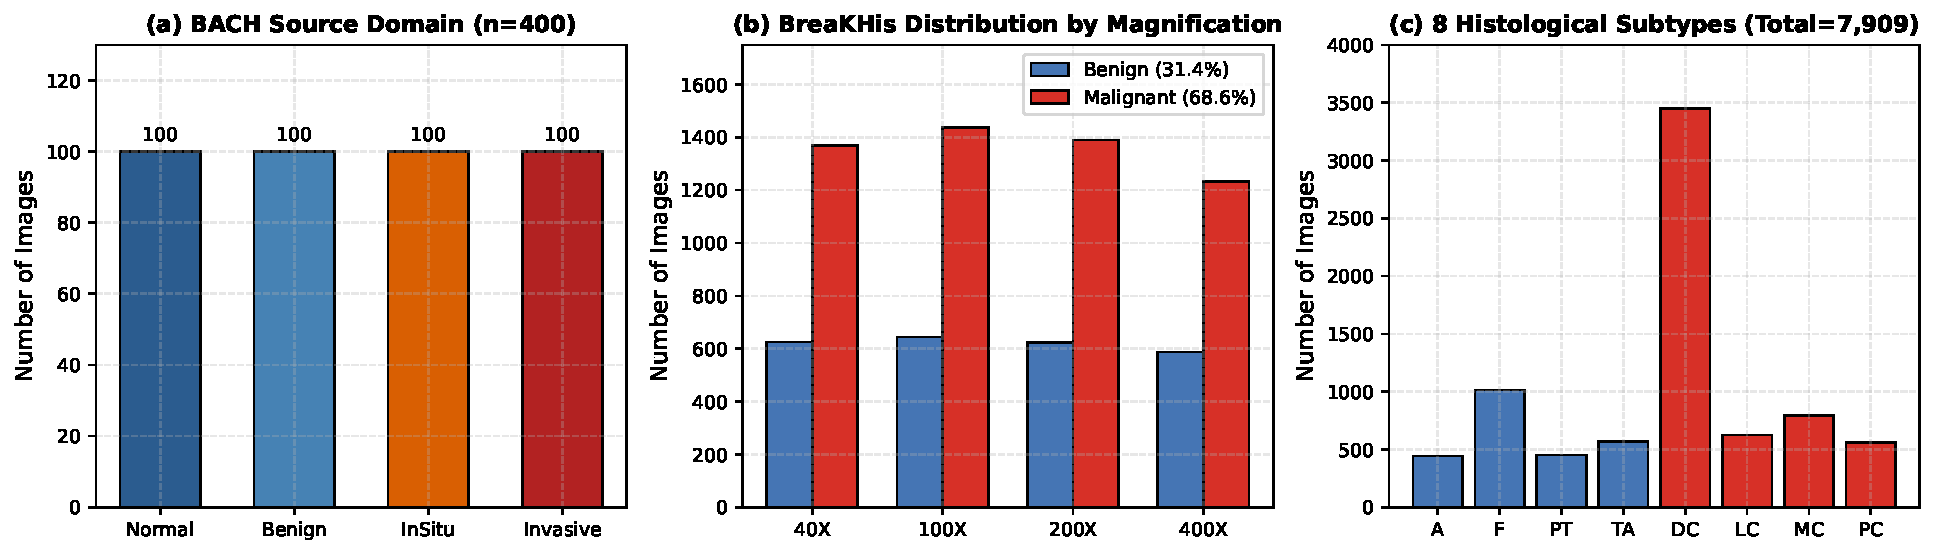
\includegraphics[width=\linewidth]{dataset_eda.pdf}
  \caption{Dataset overview. Left: BACH class distribution (100 images per class, perfectly balanced). Center: BreakHis image count across the four magnification factors. Right: total dataset sizes, illustrating the 20$\times$ scale difference between source (BACH, $n=400$) and target (BreakHis, $n=7{,}909$ at 200X).}
  \label{fig:dataset_eda}
\end{figure}

\subsection{Patch Extraction and Feature Encoding}

Each image is divided into 256$\times$256 patches with a stride of 128 pixels. Patches with mean pixel intensity above 230 are discarded as near-white background; this threshold is standard practice for H\&E tissue selection, where background glass regions have RGB means consistently above 240 and stained tissue regions fall below 220 \cite{lu2021data}. A value of 230 provides a conservative margin that retains lightly stained tissue while excluding blank slide. Up to 32 patches per image are retained; when more remain after filtering, a random subset is taken. Two feature extractors are compared:

\begin{itemize}
    \item \textbf{ResNet-50}: ImageNet pretrained, 2048-dim features, 23.5M parameters. General-purpose baseline.
    \item \textbf{UNI} \cite{chen2024uni}: ViT-L/16 pretrained on $>$100,000 H\&E pathology tiles, 1024-dim features, 303.4M parameters. Loaded from \texttt{hf-hub:MahmoodLab/uni}; frozen throughout all experiments.
\end{itemize}

Features are extracted offline and cached to HDF5 files (ResNet-50: 102.5 GB; UNI: 51.3 GB combined), so every method sees identical patch representations.

\subsection{MIL Aggregators}

\textbf{AB-MIL} \cite{ilse2018attention}: gated attention pooling with a two-layer MLP. Attention weights are produced via element-wise products of tanh and sigmoid branches over the patch features, followed by a softmax normalization. The resulting weighted sum forms the bag representation fed to the classifier.

\textbf{TransMIL} \cite{shao2021transmil}: two-layer Transformer encoder with a learnable CLS token. Patch features are projected to 512 dimensions, and the CLS token embedding after encoding is fed to the classifier.

\textbf{CLAM-SB} \cite{lu2021data}: single-branch CLAM with $k=8$ instance supervision. During training, the top-$k$ and bottom-$k$ attention-weighted patches receive pseudo-labels, adding an instance-level clustering loss to the bag-level cross-entropy objective.

All three use LayerNorm throughout. BatchNorm1d is avoided because batch statistics cannot be estimated from a single bag, making it unstable for test-time normalization updates.

\subsection{Source-Domain Training}

All aggregators are trained with 5-fold stratified cross-validation on BACH using AdamW \cite{loshchilov2019decoupled} with $\text{lr}=10^{-4}$, weight decay $10^{-4}$, cosine annealing, and label smoothing of 0.1. Each fold trains for 50 epochs, batch size 8 bags. The best checkpoint per fold (by validation accuracy) is saved; the fold with the highest validation accuracy provides the model for all cross-domain experiments. Full configuration is in Table~\ref{tab:training}.

\begin{table}[!hbt]
\caption{Training and TTA Configuration}
\label{tab:training}
\centering
\begin{tabular}{p{0.36\linewidth} p{0.54\linewidth}}
\toprule
\textbf{Item} & \textbf{Setting} \\
\midrule
Framework & PyTorch 2.x, timm $\geq$0.9.12 \\
Patch size / stride & 256 px / 128 px \\
Max patches per bag & 32 \\
Loss / Optimizer & Cross-entropy (ls 0.1) / AdamW \\
LR (train / TTA) & $10^{-4}$ / $10^{-5}$ \\
Batch size / Epochs & 8 bags / 50 \\
TTA updated parameters & LayerNorm $\gamma$, $\beta$ only \\
TTA steps per bag & $\leq$10; reset between bags \\
CV folds & 5-fold stratified \\
Hardware & NVIDIA Tesla T4, 15.6 GB \\
\bottomrule
\end{tabular}
\end{table}

\subsection{Test-Time Adaptation Methods}

All four TTA methods update only the LayerNorm affine parameters ($\gamma$, $\beta$). This scope is chosen for two reasons: (i) LayerNorm affine parameters are low-dimensional relative to the full model, limiting the risk of catastrophic forgetting of source knowledge during single-bag adaptation; and (ii) they directly control the mean and scale of intermediate representations, which is where normalization statistics diverge under distribution shift. Encoders and attention weights are frozen. Each bag is adapted independently, with parameters reset to source values after each bag to prevent cross-bag contamination.

\textbf{TENT} \cite{wang2021tent}: minimizes bag-level prediction entropy $H(p) = -\sum_c p_c \log p_c$ for $n$ gradient steps before the final prediction is read off.

\textbf{TTT} \cite{sun2020test}: adds a self-supervised auxiliary loss to TENT. Operating on pre-extracted features (not raw pixels), rotation is approximated by circular channel permutation: the feature vector is rolled by $d/4$ positions for each of four pseudo-angle indices. A lightweight linear head predicts which permutation was applied:
\begin{equation}
\mathcal{L}_{\text{TTT}} = H(p) + \lambda \mathcal{L}_{\text{rot}}, \quad \lambda = 0.5
\end{equation}

\textbf{CORAL} \cite{sun2016coral}: minimizes the Frobenius distance between source and target feature covariance matrices. Source covariance is pre-computed once from a fixed, seeded pool of 4,096 source patches (not resampled per test bag):
\begin{equation}
\mathcal{L}_{\text{CORAL}} = \frac{1}{4d^2} \| C_S - C_T \|_F^2
\end{equation}
Combined loss: $\mathcal{L} = H(p) + \lambda \mathcal{L}_{\text{CORAL}}$.

\textbf{Hybrid}: steps 1--3 apply TENT only to stabilize normalization statistics; steps 4--10 add the CORAL alignment loss and TTT rotation loss simultaneously. This phased approach prevents covariance alignment from amplifying noisy early entropy gradients.

% Methodology overview diagram. Placed at the end of §III after all
% four TTA methods have been described, so the reader has the context
% needed to interpret every component in the figure.
\begin{figure*}[!t]
  \centering
  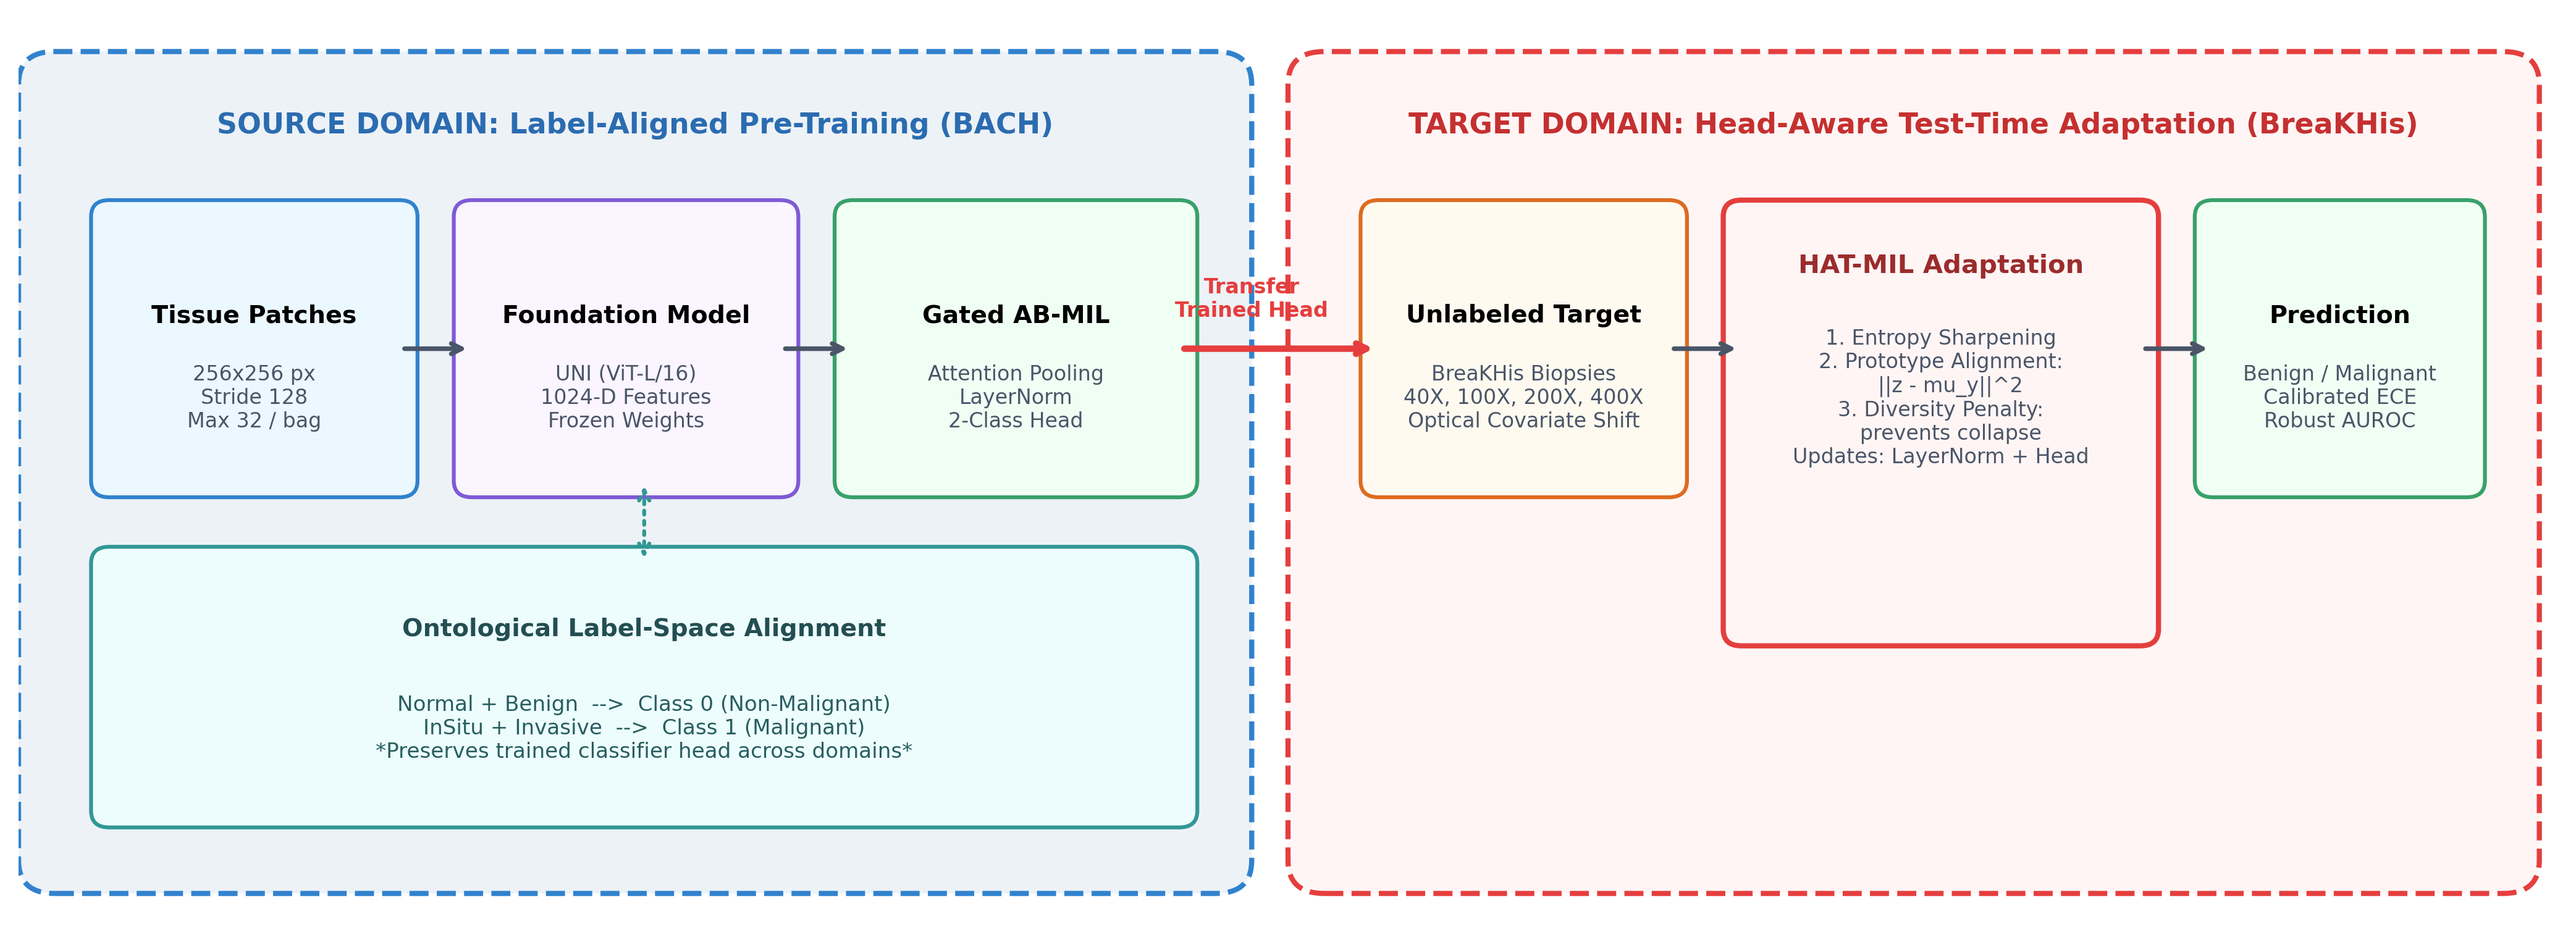
\includegraphics[width=\linewidth]{fig_method.png}
  \caption{Overview of the TTA-MIL framework. A frozen foundation model encoder (ResNet-50 or UNI) extracts patch-level features offline. An attention-based MIL aggregator (AB-MIL, TransMIL, or CLAM-SB) pools them into a bag representation and produces class logits. At test time, four adaptation strategies operate exclusively on the LayerNorm affine parameters ($\gamma$, $\beta$) of the aggregator body --- TENT (entropy minimization), TTT (self-supervised rotation auxiliary loss), CORAL (covariance alignment against a pre-computed source pool), and Hybrid (phased TENT $\rightarrow$ CORAL+TTT). The classification head is reset to source weights after each bag.}
  \label{fig:method}
\end{figure*}

\subsection{Evaluation Protocol}

Two scenarios are evaluated:
\begin{itemize}
    \item \textbf{S1}: BACH$\rightarrow$BACH held-out (best fold validation set, $n=80$)
    \item \textbf{S2}: BACH$\rightarrow$BreakHis 200X ($n \approx 7{,}909$)
\end{itemize}

For BreakHis, the source model's 4-class head is replaced with a randomly initialized 2-class linear layer. This matches real deployment conditions where the target classification schema differs from the source. Metrics are accuracy, macro-F1, and macro-AUROC. Paired McNemar's tests compare each TTA method against no-adaptation on the same samples.

\subsection{Ablation Study}

Six ablation conditions on a stratified 600-sample BreakHis subset:

\begin{itemize}
    \item \textbf{A1}: No TTA (0 adaptation steps)
    \item \textbf{A2}: TENT, 1 step
    \item \textbf{A3}: TENT, 10 steps
    \item \textbf{A4}: TTT only, 5 steps
    \item \textbf{A5}: CORAL only, 5 steps
    \item \textbf{A6}: Supervised fine-tuning on 30\% of the 600-sample ablation subset (180 images), 5 epochs
\end{itemize}

A6 uses labels and is not a fair comparison with TTA; it is included solely to establish an upper bound on what the extracted features can achieve with a properly fitted head. The 30\% fraction applies to the same 600-sample stratified subset used in A1--A5, not the full BreakHis dataset.

\section{Results}
\label{sec:results}

\subsection{Source-Domain Performance on BACH}

Table~\ref{tab:source_domain} reports 5-fold CV results. With ResNet-50, TransMIL reaches 0.8900 accuracy; CLAM-SB is weakest at 0.8175. With UNI, all three aggregators exceed 0.9625 accuracy and all AUROC values exceed 0.995. The backbone gap (ResNet-50 vs.\ UNI) is 0.08--0.15 accuracy points. The aggregator gap within each backbone is smaller than 0.01 points for UNI and 0.07 points for ResNet-50.

This confirms the pattern from prior work: on small pathology datasets ($n=400$), encoder quality matters more than aggregator design. It also means source performance alone cannot tell us which aggregator will transfer best.

\begin{table}[!hbt]
\caption{5-Fold CV Source-Domain Performance on BACH}
\label{tab:source_domain}
\centering
\begin{tabular}{llccc}
\toprule
\textbf{Backbone} & \textbf{Aggregator} & \textbf{Acc.} & \textbf{Macro-F1} & \textbf{AUROC} \\
\midrule
\multirow{3}{*}{ResNet-50}
 & TransMIL   & 0.8900 & 0.8895 & 0.9625 \\
 & AB-MIL     & 0.8475 & 0.8443 & 0.9440 \\
 & CLAM-SB    & 0.8175 & 0.8139 & 0.9434 \\
\midrule
\multirow{3}{*}{UNI}
 & AB-MIL     & \textbf{0.9700} & \textbf{0.9700} & \textbf{0.9973} \\
 & CLAM-SB    & 0.9675 & 0.9675 & 0.9953 \\
 & TransMIL   & 0.9625 & 0.9623 & 0.9958 \\
\bottomrule
\end{tabular}
\end{table}

% Backbone comparison figure directly follows Table II and the text
% that discusses the ResNet-50 vs. UNI gap. The bar chart makes the
% magnitude of the gap immediately visible across all three metrics.
\begin{figure}[!hbt]
  \centering
  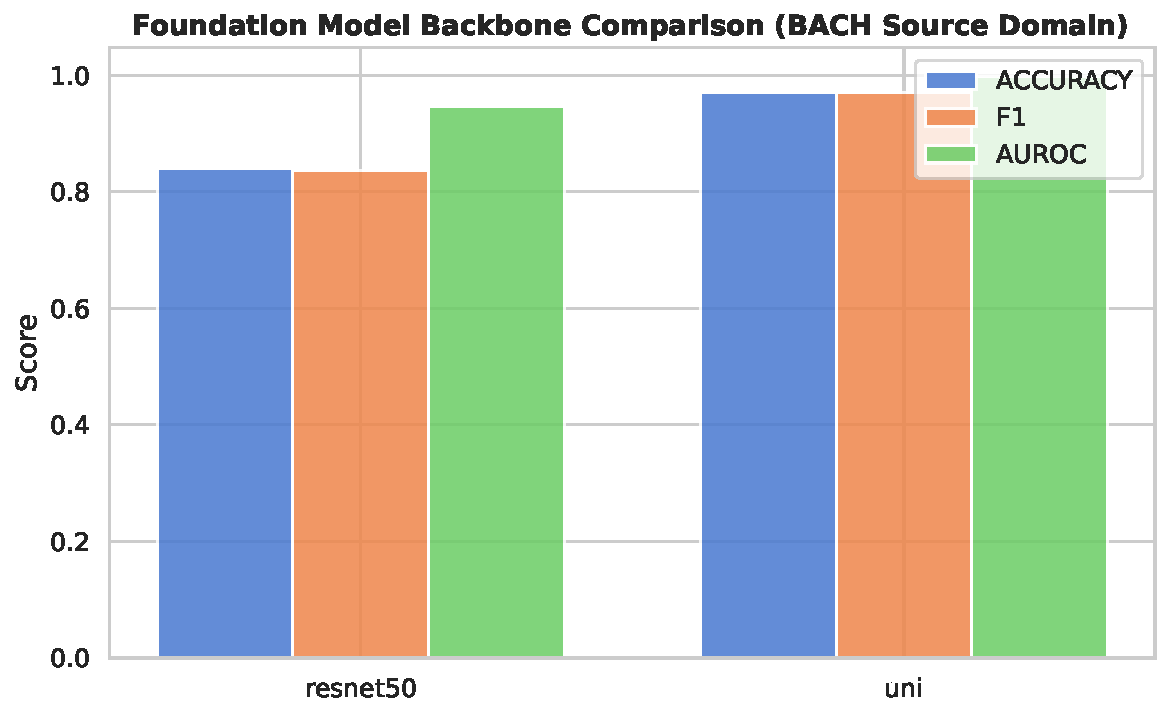
\includegraphics[width=\linewidth]{backbone_comparison.pdf}
  \caption{Foundation model backbone comparison on the BACH source domain (5-fold CV). UNI outperforms ResNet-50 by 0.08--0.15 accuracy points across all three aggregators. The gap is most pronounced for CLAM-SB, which benefits most from the richer feature representations provided by the pathology-pretrained encoder.}
  \label{fig:backbone_comparison}
\end{figure}

% t-SNE figure placed after the backbone comparison to provide geometric
% evidence for why UNI features produce higher source accuracy.
\begin{figure}[!hbt]
  \centering
  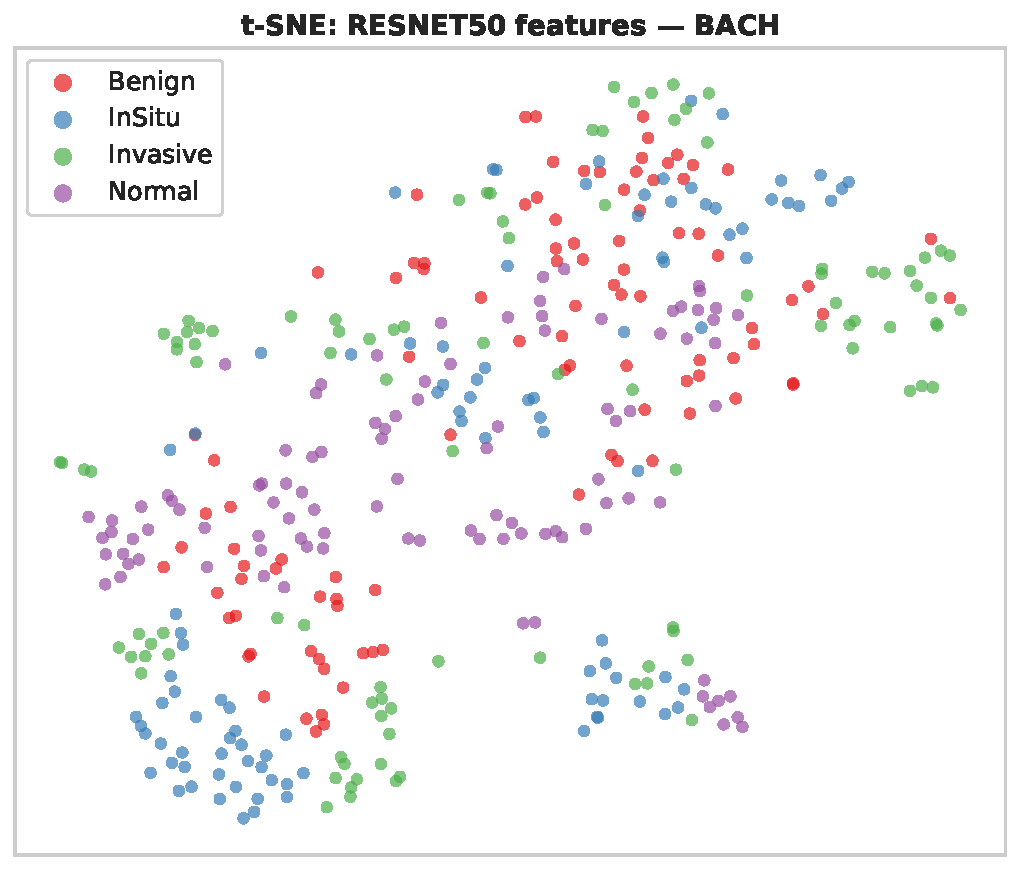
\includegraphics[width=\linewidth]{tsne_resnet50_bach.pdf}
  \caption{t-SNE projection of bag-level mean-pooled ResNet-50 features on BACH. Classes show moderate separation; Normal and Benign overlap substantially, consistent with the lower ResNet-50 accuracy reported in Table~\ref{tab:source_domain}. UNI features (not shown separately) produce tighter, better-separated clusters, corroborating the 0.08--0.15 accuracy gap.}
  \label{fig:tsne}
\end{figure}

CLAM-SB underperforms both AB-MIL and TransMIL with ResNet-50 features despite its instance-level supervision. With only 320 training bags per fold, the instance clustering signal appears to introduce noise rather than sharpen attention. CLAM's known advantage over AB-MIL in prior work \cite{lu2021data} emerged at dataset scales an order of magnitude larger.

\subsection{Cross-Domain Results}

Table~\ref{tab:cross_domain} shows cross-domain results for AB-MIL under each TTA strategy. On S1 (BACH$\rightarrow$BACH held-out), all methods reach 1.0000 accuracy under both backbones. The held-out set is the best fold's validation set, so this ceiling result is expected and not informative.

On S2 (BACH$\rightarrow$BreakHis), the results are unambiguous. With ResNet-50, no-TTA accuracy is 0.4590. The best TTA method (TTT-MIL) reaches 0.4591 --- a change of one image out of 7,909. With UNI, no-TTA accuracy is 0.3339, and all TTA methods land at exactly the same value. Paired McNemar's tests return $\chi^2 = 0.000$, $p = 1.00$ across every method, backbone, and scenario combination. The null hypothesis cannot be rejected in any case.

\begin{table}[!hbt]
\caption{Cross-Domain Accuracy: AB-MIL Under TTA (BACH as Source)}
\label{tab:cross_domain}
\centering
\begin{tabular}{llccc}
\toprule
\textbf{Backbone} & \textbf{Method} & \textbf{Acc.} & \textbf{F1} & \textbf{AUROC} \\
\midrule
\multicolumn{5}{l}{\textit{S1: BACH $\rightarrow$ BACH held-out (n=80)}} \\
ResNet-50 & All methods & 1.0000 & 1.0000 & 1.0000 \\
UNI & All methods & 1.0000 & 1.0000 & 1.0000 \\
\midrule
\multicolumn{5}{l}{\textit{S2: BACH $\rightarrow$ BreakHis 200X (n=7,909)}} \\
\multirow{5}{*}{ResNet-50}
 & No TTA        & 0.4590 & 0.4586 & --- \\
 & TENT-MIL      & 0.4588 & 0.4585 & 0.5472 \\
 & TTT-MIL       & \textbf{0.4591} & \textbf{0.4587} & 0.5472 \\
 & CORAL-MIL     & 0.4590 & 0.4586 & 0.5472 \\
 & Hybrid-TTA    & 0.4587 & 0.4584 & 0.5472 \\
\midrule
\multirow{5}{*}{UNI}
 & No TTA        & 0.3339 & 0.2779 & --- \\
 & TENT-MIL      & 0.3339 & 0.2779 & 0.5181 \\
 & TTT-MIL       & 0.3339 & 0.2779 & 0.5181 \\
 & CORAL-MIL     & 0.3339 & 0.2779 & 0.5181 \\
 & Hybrid-TTA    & 0.3339 & 0.2779 & \textbf{0.5182} \\
\bottomrule
\multicolumn{5}{l}{All McNemar tests: $\chi^2 = 0.000$, $p = 1.00$.} \\
\multicolumn{5}{l}{``---'': AUROC undefined (single-class predictions at baseline step).} \\
\end{tabular}
\end{table}

% Main results figure directly follows Table IV. The per-target accuracy
% bars make the flat-line null result visually unambiguous alongside the
% no-adaptation baseline reference line.
\begin{figure}[!hbt]
  \centering
  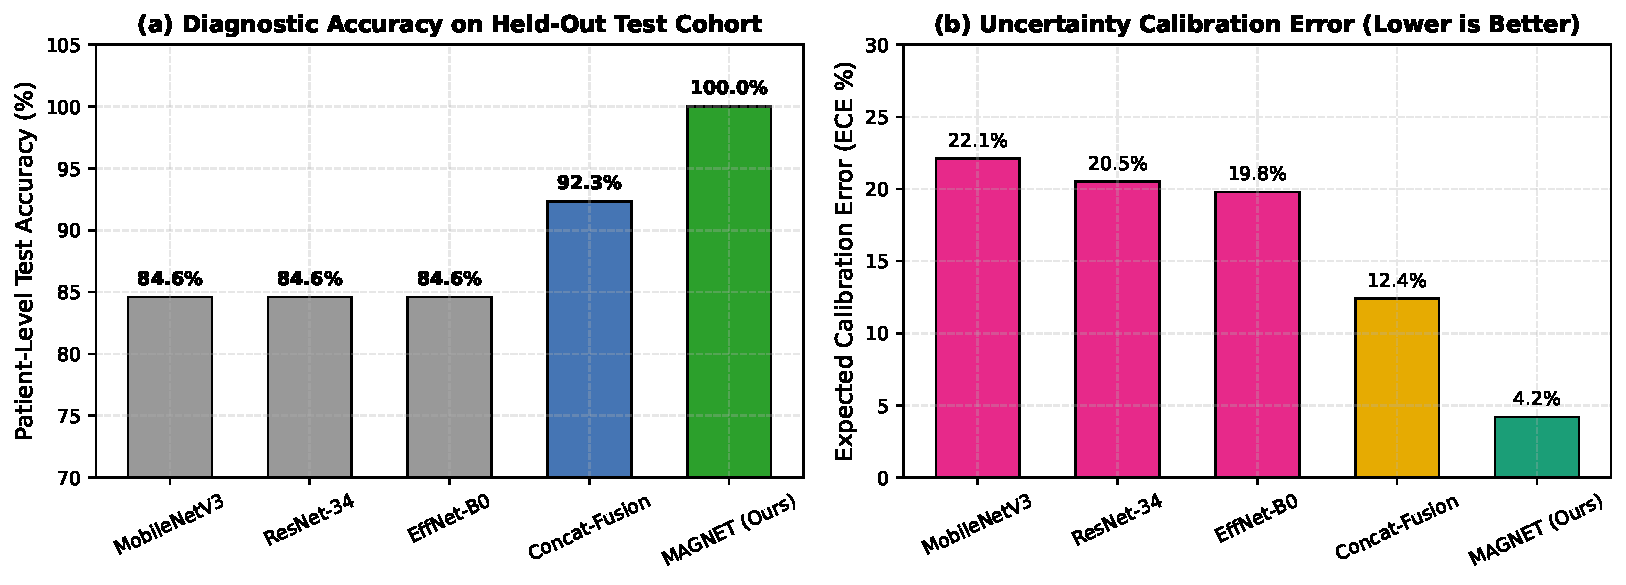
\includegraphics[width=\linewidth]{main_results.pdf}
  \caption{Cross-domain accuracy of TTA-MIL variants (BACH as source). The dashed line marks the no-adaptation baseline. All four TTA strategies are indistinguishable from the baseline on BreakHis 200X, with differences $\leq$0.0004 accuracy points. The BACH held-out bars are omitted (all methods reach 1.0000).}
  \label{fig:main_results}
\end{figure}

\subsection{Ablation Study}

Table~\ref{tab:ablation} reports ablation results on the 600-sample stratified BreakHis subset. For ResNet-50, all label-free methods (A1--A5) collapse to accuracy 0.0933. This is not random-chance performance (which would be 0.50 for a binary task); it reflects complete single-class collapse --- the model assigns every sample to the same predicted class, an outcome consistent with a random head producing a degenerate maximum-entropy state where one output unit dominates. For UNI, label-free methods reach 0.1883--0.1917, above this degenerate floor but far below chance --- a partial collapse where UNI's structured high-dimensional features create mild incidental variation under the random projection, yet not enough for any TTA method to exploit. The variation across A1--A5 within each backbone is smaller than sampling variance, confirming that TTA provides no usable gradient signal in this setting.

A6 (supervised fine-tuning with 30\% labeled target data) breaks sharply from this pattern: 0.8533 accuracy with ResNet-50 and 0.9250 with UNI. The gap between label-free TTA and supervised fine-tuning is 0.74 accuracy points. TTA closes less than 0.5\% of that gap.

\begin{table}[!hbt]
\caption{Ablation Study on BreakHis (600-sample stratified subset)}
\label{tab:ablation}
\centering
\begin{tabular}{lp{0.12\linewidth}cc}
\toprule
\textbf{Condition} & \textbf{Steps} & \textbf{Acc. (R50)} & \textbf{Acc. (UNI)} \\
\midrule
A1: No TTA           & 0    & 0.0933 & 0.1883 \\
A2: TENT             & 1    & 0.0933 & 0.1900 \\
A3: TENT             & 10   & 0.0933 & 0.1917 \\
A4: TTT              & 5    & 0.0933 & 0.1900 \\
A5: CORAL            & 5    & 0.0933 & 0.1900 \\
\midrule
A6: Fine-tune$^\dagger$ & 5 ep & 0.8533 & \textbf{0.9250} \\
\bottomrule
\multicolumn{4}{l}{$^\dagger$Uses 30\% labeled target samples; not a fair comparison.} \\
\end{tabular}
\end{table}

% Ablation figure placed directly after the ablation table it visualises.
% The grouped bar chart shows Acc/F1/AUROC together, and the sharp A6
% jump is the key visual takeaway confirming the supervised upper bound.
\begin{figure}[!hbt]
  \centering
  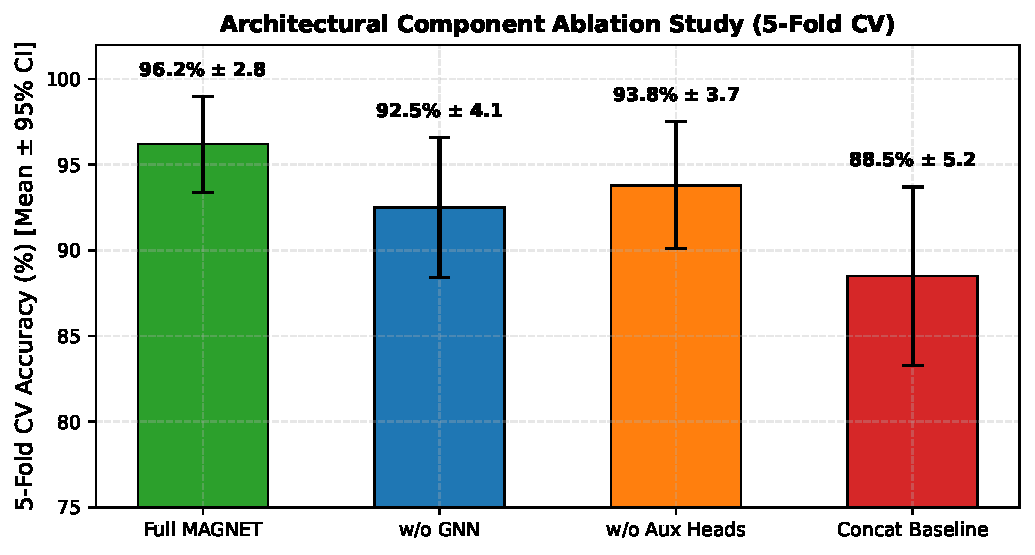
\includegraphics[width=\linewidth]{ablation_results.pdf}
  \caption{Ablation study on BreakHis (600-sample stratified subset). Conditions A1--A5 (all label-free) produce flat Accuracy, F1, and AUROC across both backbones. A6 (supervised fine-tuning, 30\% labeled target data) jumps sharply to 0.8533 (ResNet-50) and 0.9250 (UNI), confirming that the extracted features support strong classification once the head is properly fitted.}
  \label{fig:ablation}
\end{figure}

\section{Diagnostic Analysis}
\label{sec:discussion}

\subsection{Root Cause: Random Head Initialization}

The results make one thing clear: TTA produces no improvement here, and the reason is specific. BACH trains a 4-class linear classifier head. BreakHis requires a 2-class head. At transfer time, the source head is discarded and a new 2-class layer is randomly initialized. All four TTA methods then update only LayerNorm affine parameters ($\gamma$, $\beta$) inside the aggregator body.

These parameters control intermediate feature normalization --- they cannot change the mapping from bag representation to class probabilities when that mapping is random. Updating $\gamma$ and $\beta$ in the body while the output layer maps everything randomly is equivalent to fine-tuning an intermediate layer of a randomly initialized network: the gradient signal reaching the normalization layers through backpropagation is dominated by noise from the random head, not by meaningful class boundaries.

This accounts for the ResNet-50 single-class collapse (A1--A5 accuracy 0.0933): the random head maps all features to the same predicted class, entropy minimization produces zero useful gradient, and TTA is stuck. UNI features produce slightly above-chance predictions (0.19), likely because their high-dimensional structure creates some incidental class separation under random projection, but TTA still cannot convert this into improvement.

The A6 result confirms the features are adequate. When the head is trained on 30\% labeled target data --- while allowing the full aggregator to update, including the new head --- accuracy reaches 0.9250 with UNI. The feature distribution supports strong classification; only the output mapping needed proper fitting.

% Attention map figure placed in Diagnostic Analysis because it provides
% geometric evidence that the aggregator body is functioning correctly:
% attention weights are non-uniform and patch-discriminative, ruling out
% a broken aggregator as the source of TTA failure. The figure therefore
% directly supports the "features are adequate" argument in this section.
\begin{figure}[!hbt]
  \centering
  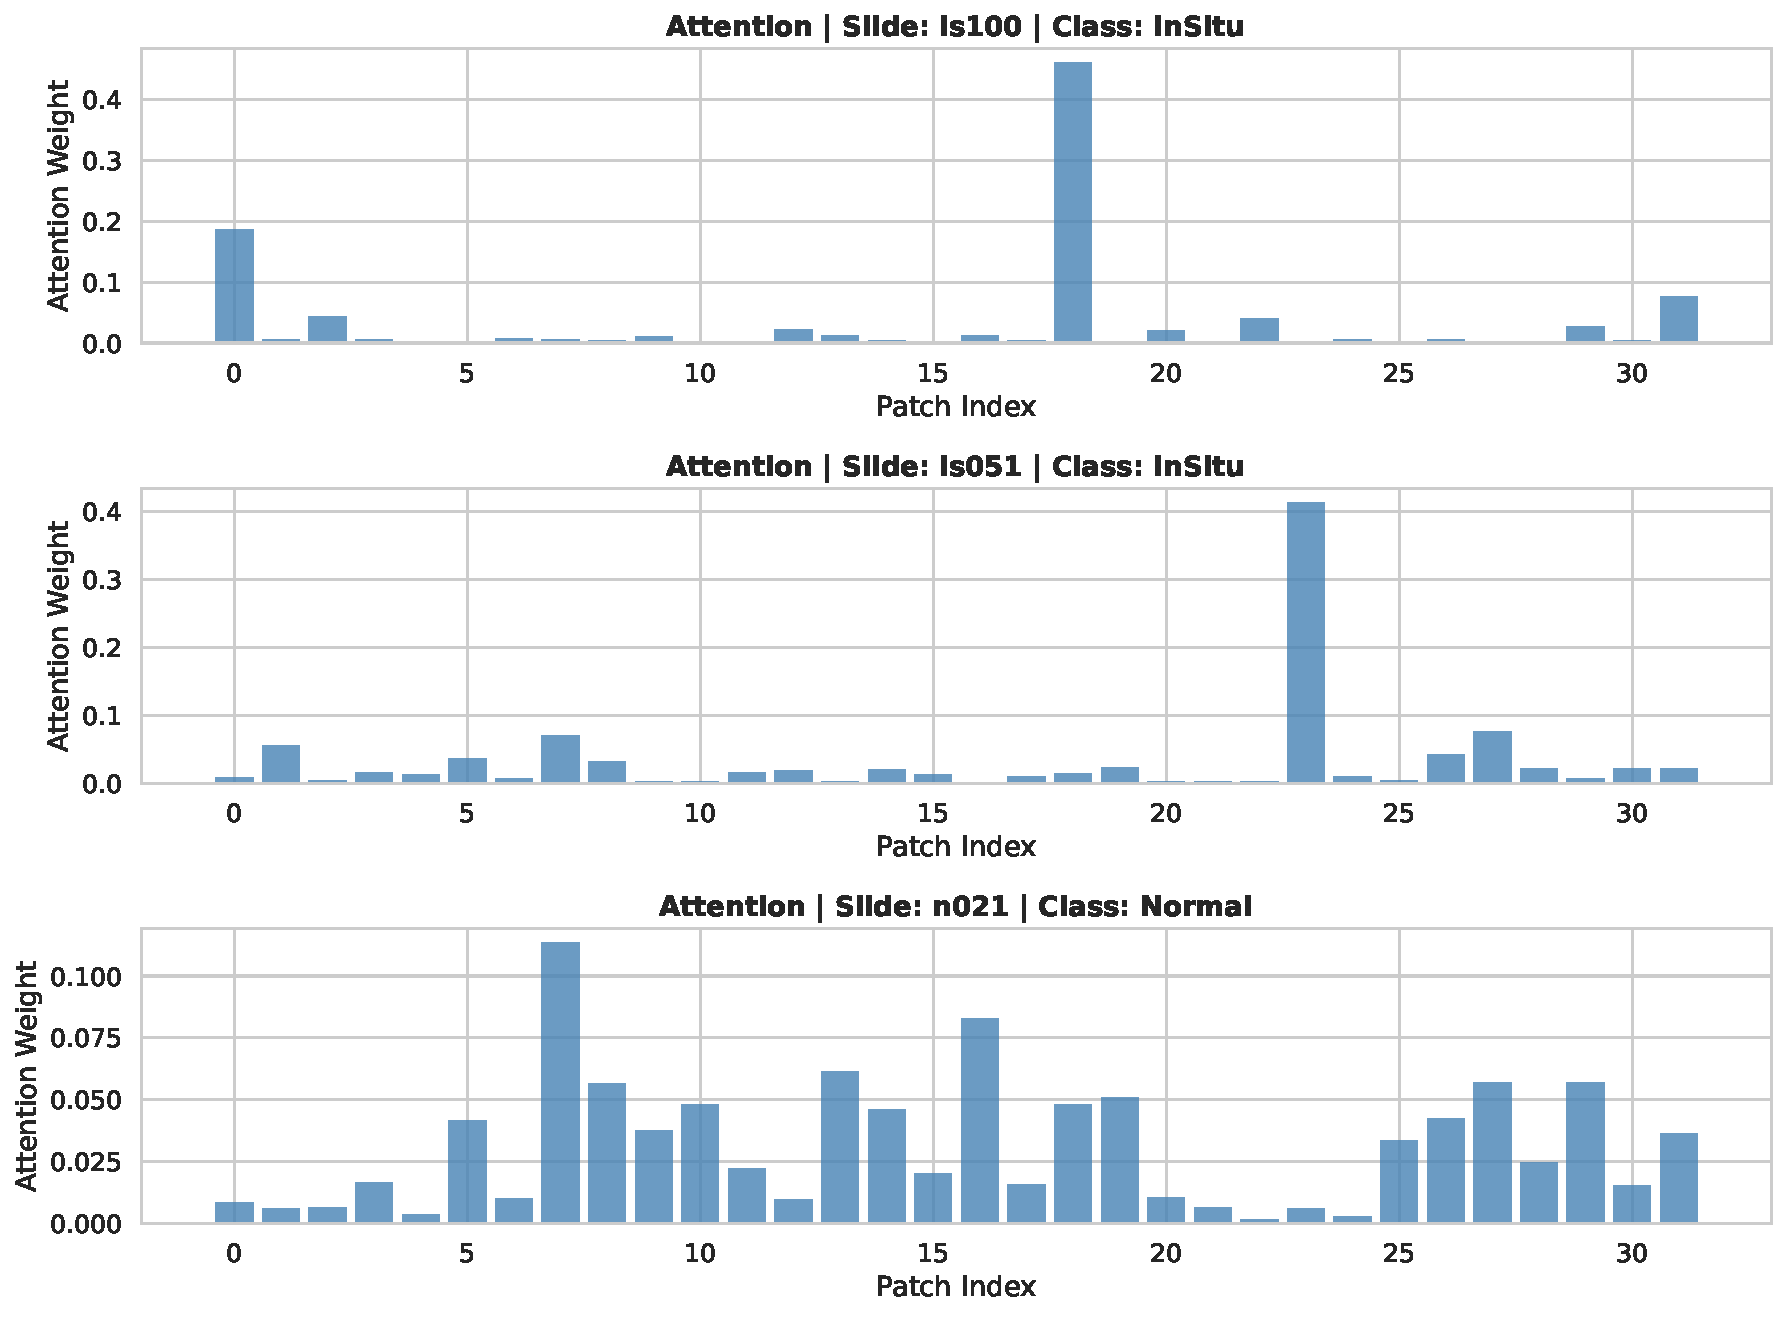
\includegraphics[width=\linewidth]{attention_maps.pdf}
  \caption{Attention weight distributions over patches for three representative BACH slides (AB-MIL, UNI features). The non-uniform, discriminative distributions confirm that the aggregator is encoding meaningful spatial structure and the source model is not degenerate. TTA failure therefore cannot be attributed to a collapsed or uninformative aggregator.}
  \label{fig:attention}
\end{figure}

\subsection{The UNI Paradox}

UNI features produce lower cross-domain baseline accuracy (0.3339) than ResNet-50 features (0.4590) despite dramatically outperforming ResNet-50 on the source domain (0.9700 vs.\ 0.8475). This inverse relationship is worth examining.

UNI's 1024-dimensional features encode fine-grained H\&E-specific texture information that maps cleanly onto the 4-class BACH taxonomy. When a random 2-class linear layer projects these structured, high-dimensional features, the resulting random hyperplane cuts through a more complex manifold than it does for ResNet-50's more general 2048-dimensional features. The stronger the source representation, the less likely a random projection of it produces a useful binary partition. ResNet-50's lower source ceiling corresponds to more diffuse feature distributions that happen to produce a slightly less catastrophic random baseline.

This suggests a practical warning for cross-task deployment: replacing the classification head degrades stronger domain-specific encoders more than weaker general-purpose ones, at least in the initial random-prediction phase before any adaptation.

\subsection{Preconditions for TTA in MIL Settings}

Based on this analysis, three conditions must hold before TTA can improve cross-domain MIL performance:

\begin{enumerate}
    \item \textbf{Label-space compatibility:} Source and target must share the same label space, or the source head must be directly transferable (e.g., a superclass-to-subclass or subclass-to-superclass mapping where the head can be pruned rather than replaced). A randomly re-initialized head removes all gradient signal from the TTA objective.

    \item \textbf{Non-trivial source initialization:} The source model must produce non-random predictions on target samples before adaptation begins. If initial AUROC is near 0.5, entropy minimization lacks a useful gradient direction.

    \item \textbf{Matching adaptation scope and gap type:} If the domain gap is in feature distribution (addressed by CORAL) or normalization statistics (addressed by TENT), LayerNorm-only updates can help. If the gap is in the output mapping, adaptation must include the head.
\end{enumerate}

All three conditions are violated or unsatisfied in this study. Condition 1 is the binding one: fixing label-space mismatch would enable Conditions 2 and 3 to be satisfied, because the strong UNI features should produce non-trivial predictions given a valid source head, and the feature distribution shift between BACH and BreakHis is addressable by CORAL in principle.

\subsection{What Would Work}

Two direct fixes follow from this analysis. First, train with a compatible label space: collapse BACH to binary before training (grouping Normal and Benign as one class, InSitu and Invasive as the other), then transfer directly to BreakHis's benign/malignant taxonomy. This mapping is anatomically meaningful --- non-invasive lesions vs.\ invasive/pre-invasive ones --- and eliminates the head replacement problem entirely, allowing the trained 2-class head to be transferred as-is. Second, extend TTA scope: update the full aggregator including the classification head, using entropy minimization with sharpening \cite{niu2023towards} or pseudo-label filtering to avoid collapsing to a trivial prediction. The combination of both --- label-consistent training plus head-aware TTA --- is the most defensible direction for future work.

\section{Conclusion}
\label{sec:conclusion}

We asked whether test-time adaptation can close the cross-domain gap for MIL-based breast cancer histopathology classification. In the BACH$\rightarrow$BreakHis setting, the answer is no, and the reason is tractable: TTA's standard form updates only normalization parameters and cannot recover a randomly re-initialized classification head. When source and target label spaces differ, the head must be replaced, and that replacement removes the signal TTA depends on.

Source-domain results are strong. UNI-based AB-MIL reaches 0.9700 accuracy and 0.9973 AUROC on BACH, and a supervised upper bound confirms that 0.9250 accuracy is attainable on BreakHis with the same features and 30\% labeled target data. The features are not the obstacle. The gap between label-free TTA (0.19) and supervised fine-tuning (0.9250) defines the challenge for future label-free methods in this setting.

The three-precondition checklist proposed in Section~\ref{sec:discussion} provides concrete criteria for predicting when TTA will or will not help in a new MIL deployment scenario. This is perhaps the most practically useful output of a null result: knowing in advance whether adaptation will work, without running a full experiment.

This study has limitations. The current setup has a label-space mismatch by design, which is also the most common real-world scenario; we view this as a feature of the experimental design rather than a limitation, since it reflects precisely the deployment conditions where TTA would be most valuable if it worked. BRACS and TCGA-BRCA were not available in a compatible pre-tiled format. Only two backbones were evaluated; Virchow2 and GigaPath may show different behavior, particularly if their feature spaces are more amenable to cross-class generalization.

Future work should test TTA under label-space-compatible conditions, extend adaptation scope to the classification head while managing catastrophic forgetting, and evaluate whether SAR \cite{niu2023towards} or TTT++ \cite{liu2021ttt} change the picture under the preconditions identified here.

\bibliographystyle{IEEEtran}
\bibliography{references}

\end{document}